\section{Software Verification}

Software programs are becoming increasingly complex. 
With the rise in complexity and technological advancements, components within a software have become susceptible to various erroneous conditions. 
Software verification have been perceived as a solution for the problems arising in the software development cycle. 
Software verification is primarily verifying if the specifications are met by the software\cite{ghezzi2002fundamentals}.

There are two fundamental approaches used in software verification - dynamic and static software verification\cite{ghezzi2002fundamentals}. 
Dynamic software verification is performed in conjunction with the execution of the software. 
In this approach, the behavior of the execution program is checked- commonly known as Test phase. 
Verification is succeeding phase also known as Review phase. 
In dynamic verification, the verification adheres to the concept of test and experimentation. 
The verification process handles the test and behavior of the program under different execution conditions. 
Static software verification is the complete opposite of the previous approach. 
The verification process is handled by checking the source code of the program before its execution. 
Static code analysis is one such technique which uses a similar approach. 

The verification of software can also be classified in perspective of automation - manual verification and automated verification. 
In manual verification, a reviewer manually verifies the software. 
Whereas in the latter approach, a script or a framework performs  verification. 

Software verification is a very broad area of research. 
This thesis work is focused on automated software verification for multithreaded programming. 

\section{Multithreaded Programming \label{multi_thread}}

Computing power has grown over the years. 
Advancements are made in the domain of computer architecture by moving the computing power from single-core to multi-core architecture. 
With such advancement, there were needs to adapt the programming designs from a serialized execution to more parallelizable execution. 
Various parallel programming models were perceived to accommodate the perceived progression. 
Multithreaded programming model was one of the designs considered for the performance boost in computing\cite{carver2005modern}. 

Threads are small tasks executed by a scheduler of an operating system, where the resources such as the processor, TLB (Translation Lookaside Buffer), cache, etc., are shared between them. 
Threads share the same address space and resources. 
Multithreading addresses the concept of using multiple threads for having concurrent execution of a program on a single or multi-core architectures. 
Inter-thread communication is achieved by shared memory. 
Mapping the threads to the processor core is done by the operating system scheduler. 
Multithreading is only supported in operating systems which has multitasking feature. 

Advantages of using multithreading include: 
\begin{itemize}
\item	Fast Execution
\item	Better system utilization
\item	Simplified sharing  and communication
\item 	Improved responsiveness - Threads can overlap I/O and computation.
\item	Parallelization
\end{itemize}

Disadvantages:
\begin{itemize}
\item	Race conditions
\item	Deadlocks with improper use of locks/synchronization
\item	Cache misses when sharing memory
\end{itemize}

\section{Concurrency Bugs \label{con_bugs}}

Concurrency bugs are one of the major concerns in the domain of multithreaded environment. 
These bugs are very hard to find and reproduce. 
Most of these bugs are propagated from the mistakes made by the programmer\cite{lopez2017study}. 
Some of these concurrency bugs include:
\begin{itemize}
\item	Data Race
\item 	Order violation
\item	Deadlock
\item	Livelock
\end{itemize}

Non-deterministic behavior of threads is one of the reasons for having the among mentioned bugs. 
Data race and order violation are classified as race condition bugs. 
Whereas, deadlock and livelock are classified as lack of progress bugs. 

\subsection{Race Condition}

Race condition is one of the most class of common concurrency problems.  
The problem arises, when there are concurrent reads and writes of a shared memory location. 
As stated above, the problem occurs with non-deterministic execution of threads. 

Consider the following example, you have three threads and they share two variables \emph{x} and \emph{y} \cite{carver2005modern}. 
The value of \emph{x} is initially 0. 

\begin{table}[h]
\centering
\begin{tabular}{*{3}{c}}
Thread 1 & Thread 2 & Thread 3 \\
\hline
 (1) \emph{x} = 1 & (2) \emph{x} = 2 & (3) \emph{y} = \emph{x}\\
\end{tabular}
\caption{Race condition example}
\label{race_cond}
\end{table}

If the statements (1), (2) and (3) were executed as a sequential program. 
The value of \emph{y} would be 2. 
When the same program is split to three threads as shown in the above Table~\ref{race_cond}, the output of \emph{y} becomes unpredictable. 
The possible values of \emph{y} = \{0,1,2\}. 
The non-deterministic execution of the threads makes the output of \emph{y} non-deterministic. 
Table~\ref{poss_exec} depicts possible executions for the above multithreaded execution. 

\begin{table}[h]
\centering
\begin{tabular}{*{2}{c}}
Execution Order & Value of \emph{y} \\
\hline
 (3),(1),(2)& 0\\
 (3),(2),(1)& 0\\
 (2),(1),(3)& 1\\
 (1),(3),(2)& 1\\
 (1),(2),(3)& 2\\
 (2),(3),(1)& 2\\
\end{tabular}
\caption{Possible executions}
\label{poss_exec}
\end{table}

The above showcased problem is classified as race condition bug. 
Ordered execution of reads and writes can fix the problem. 

\subsection{Lack Of Progress}

Lack of progress is another bug class observed in multithreaded programs. 
Some of the bugs under this class include deadlocks and livelocks. 

\subsubsection{Deadlock}

Deadlock is a state in which each thread in thread pool is waiting for some other thread to take action. 
In terms of multithreaded programming environment, deadlocks occur when one thread waits on a resource locked by another thread, which in turn is waiting for another resource locked by another thread. 
If a thread is unable to change its state indefinitely because the resource requested by it are being held by another thread, then the entire system is said to be in deadlock\cite{chaki2005concurrent}. 

%----Example Picture depicting deadlock---
\tikzstyle{thread} = [circle, minimum size=.5cm, text centered, draw=black, fill=white!30]
\tikzstyle{resource} = [rectangle, minimum width=1cm, minimum height=1cm, text centered, draw=black, fill=white!30]

\begin{figure}[h]
\centering
\begin{tikzpicture}[node distance=2cm]
%Resources
\node (R1) [resource] {R$_1$};
\node (R2) [resource,right of=R1,xshift =1cm] {R$_2$};
\node (R3) [resource,right of=R2,xshift =1cm] {R$_3$};

%Threads
\node (T1) [thread,below of=R1,xshift =1cm] {T$_1$};
\node (T2) [thread,below of=R2,xshift =1cm] {T$_2$};
\node (T3) [thread,below of=R3,xshift =1cm] {T$_3$};

%Arrows
\draw [->,thick] (R1.south) -- (T1);
\draw [->,thick] (R2.south) -- (T2);
\draw [->,thick] (R3.south) -- (T3);
\draw [->,thick] (T1) -- (R2.west);
\draw [->,thick] (T2) -- (R3.west);
\draw [->,thick] (T3.south) to [out=220,in=230] (R1.west);

\end{tikzpicture}
\caption{Dead Lock Example}
\label{deadlock_example}
\end{figure}

In the example depicted in Fig~\ref{deadlock_example}, we have three threads T$_1$, T$_2$, T$_3$ and three resource instances R$_1$, R$_2$, R$_3$. 
The figure depicts hold and wait by each threads. 
Thread T$_1$ holds resource R$_1$ and waits for the acquisition of resource R$_2$ from thread T$_2$. 
T$_2$ cannot relinquish resource R$_2$, unless it acquires resource R$_3$ for its progress. 
But, resource R$_3$ is acquired by T$_3$ and is waiting for R$_1$ from T$_1$. 
Thus, making a circular wait of resources. 
This example clearly explains the dependency of resources for the respective thread progress. 

Deadlock can occur if all the following conditions are met simultaneously.

\begin{itemize}
\item	Mutual exclusion
\item	Hold and wait
\item	No preemption
\item	Circular wait
\end{itemize}

These conditions are known as Coffman conditions\cite{coffman_cond}.

Deadlock conditions can be avoided by having scheduling of threads in a way to avoid the resource contention issue.

\subsubsection{Livelock}

Livelock is similar to deadlock, except the state of threads change constantly but, with none progressing. 
Livelock is special case of resource starvation of threads/processes. 
Some deadlock detection algorithms are susceptible to livelock conditions when, more than one process/thread tries to take action\cite{lopez2017study}\cite{chaki2005concurrent}. 
The above mentioned situation can be avoided by having one priority process/thread taking up the action. 

\section{Model Checking \label{model_check}}

From section~\ref{con_bugs}, it is very clear that there needs to be verification for multithreaded programs. 
The verification solutions range from detecting causality violations to correctness of execution\cite{d2008survey}. 
Model checking is an example of such a technique. 
It is used for automatically verifying correctness properties of finite-state concurrent systems\cite{model_check}\cite{berard2013systems}. 
This technique has a number of advantages over traditional approaches that are based on simulation, testing and deductive reasoning. 
When solving a problem algorithmically, both the model of the system and the specification are forumulated in a precise mathematical language. 
Finally, the problem is formulated as a task in logic, namely to verify whether a given structure adheres to a given logical formula.  
The technique has been successfully used in practice to verify complex sequential designs and communication protocols\cite{model_check}. 
Model checker tries to verify all possible states of a system in a brute force manner\cite{model_checking_principles}. 
Thus, making \emph{state explosion} as one of the major challenges, which is discussed in detail in section~\ref{state_exp_prob}.  
Model checking tools usually verify partial specification for liveness and safety properties\cite{d2008survey}. 
Model checking algorithms generate set of states from the instructions of a program, which are later analyzed. 
There is a need to store these states for asserting the number of visits made them are atmost once. 
There are two methods commonly used to represent states:
\begin{itemize}
\item	Explicit-state model checking
\item	Symbolic model checking
\end{itemize}

\paragraph{Advantages of using model checking:} 
\begin{itemize}
\item	Generic verification approach used across various domains of software engineering.
\item 	Supports partial verification, more suited for assessment of essential requirements for a software.
\item 	Not vulnerable to the likelihood that an error is exposed. 
\item  	Provides diagnostic information thus, making it suitable for debugging purposes. 
\item	Based on graph theory, data structures and logic thus, making it `sound and mathematical underpinning'. 
\item 	Easy to understand and deploy. 

\end{itemize}

\paragraph{Disadvantages of using model checking:}
\begin{itemize}
\item	State explosion problem.
\item	Appropriate for control-intensive applications rather than data-intensive applications. 
\item	Verifies system model and not the actual system. 
\item	Decidability issues when considering abstract data types or infinite state systems.
\end{itemize}

\subsection{State explosion problem \label{state_exp_prob}}

The state space of a program is exponential in nature when it comes to number of variables, inputs, width of the data types, etc,. 
Presence of function calls and dynamic memory allocation makes it infinite\cite{d2008survey}. 
Concurrency makes the situation worse by having interleaving of threads during execution. 
Interleaving generates exponential number of ways to execute a set of statements/instructions. 
Thus, having an explosion in state space. 
There are various techniques used to avoid the \emph{state explosion problem}. 
 
\subsection{Explicit-state Model Checking}

Explicit-state model checking methods recursively generate successors of initial states by constructing a state transition graph. 
Graphs are constructed using depth-first, breadth-first or heuristic algorithms. 
Erroneous states are determined `on the fly' thus, reducing the state space. 
A property violation on the newly generated states are regarded as erroneous states. 
Hash tables are used for indexing the explored states. 
If there is insufficient, memory lossy compression algorithms are used to accommodate the storage of hash tables\cite{d2008survey}. 
Explicit-state techniques are more suited for error detection and handling concurrency. 

\subsection{Symbolic Model Checking}

Symbolic model checking methods manipulate a set of states rather than single states. 
Sets of states are represented by formulae in propositional logic. 
It can handle much larger designs with hundreds of state variables. 
Symbolic model checking uses different model checking algorithms: fix-point model checking(mainly for CTL), bounded model checking(mainly for LTL), invariant checking, etc,. 
Two main symbolic techniques used - Binary Decision Diagrams(BDD) and Propositional Satisfiability Checkers(SAT solvers). 
BDDs are traditionally used to represent boolean functions. 
A BDD is obtained from a Boolean decision tree by maximally sharing nodes and eliminating redundant nodes. 
However, BDDs grow very large. 
The issues in using finite automata for infinite sets are analogous. 
Symbolic representations such as propositional logic formulas are more memory efficient, at the cost of computation time. 
Symbolic techniques are suitable for proving correctness and handling state-space explosion due to program variables and data types.


\subsection{Partial Order Reduction}

Partial Order Reduction(POR) is a technique used for reducing the size of state space to be searched by a model checking algorithm\cite{por10yrs}. 
This technique exploits the independence of concurrently executed events. 
Two events are independent of each other when executing them either order results in the same global state\cite{model_check}. 
A common model for representing concurrent software is to have it depicted as interleaving model. 
In interleaving model, we have a single linear execution of the program arranged in an interleaved sequence. 
Concurrently executed events appear to be ordered arbitrarily to each other. 
Considering all interleaving sequences would lead to extremely large state space. 
Constructing full state graph would make the fitting into the memory difficult. 
Therefore, a reduced state graph construction is used in this technique. 
 
POR exploits the commutativity of concurrently executed transitions, which would result in the same state. 
Fig ~\ref{commutativity_example} depicts the commutativity behavior. 
$S$, $S_1$, $S_2$ and $R$ are various states of a given program and $\alpha_1$, $\alpha_2$ represents various transitions. 
Consider two paths $P_1$ and $P_2$. 
$P_1 = S \rightarrow S_1 \rightarrow  R$ and $P_2 = S \rightarrow S_2 \rightarrow  R$. 
$P_1$ and $P_2$ reaches the same final state $R$. 
Thus, showing us that commutativity of transitions $\alpha_1$, $\alpha_2$ on the given example. 





%----Example Picture depicting deadlock---
\tikzstyle{state} = [circle, minimum size=1cm, text centered, draw=black, fill=white!30]

\begin{figure}[h]
\centering
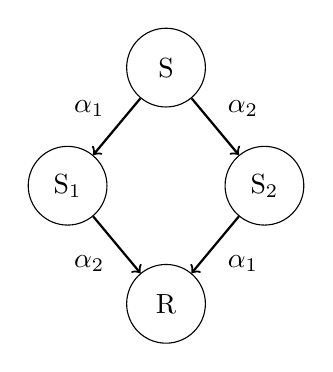
\begin{tikzpicture}[node distance=1.5cm]

%Threads
\node (S) [state] {S};
\node (S1) [state,below of=S,xshift =-1.25cm] {S$_1$};
\node (S2) [state,below of=S,xshift =1.25cm] {S$_2$};
\node (R) [state,below of=S2,xshift =-1.25cm] {R};

%Arrows
\draw [->,thick] (S) to node [above] {$\alpha_1\ \ \ \ \ \ $} (S1);
\draw [->,thick] (S) to node [above] {$\ \ \ \ \ \ \alpha_2$} (S2);
\draw [->,thick] (S1) to node [below] {$\alpha_2\ \ \ \ \ \ $}  (R);
\draw [->,thick] (S2) to node [below] {$\ \ \ \ \ \ \alpha_1$}  (R);

\end{tikzpicture}
\caption{Commutativity Example}
\label{commutativity_example}
\end{figure}

$B_r \subset B_f$

$B_f$ represents the behaviors of full state graph and $B_r$ represents set of behaviors of reduced graph. 
Partial order reduction derives its motivation from the early versions of algorithms used for partial order modeling of program execution. 
POR is described as model checking using representatives\cite{por_repr}. 
Verification is performed using representatives from equivalence classes of behaviors. 

The transitions of a system play a major role in the POR. 
POR is based on the dependency relation that exists between the transitions of a systems. 
A transition $\alpha \in T$ is enabled in a state $s$, if there is a state $s'$ such that $\alpha(s, s')$ holds. 
Otherwise, $\alpha$ is disabled in $s$. 
The set of transitions enabled in $s$ is $enabled(s)$. 
A transition $\alpha$ is deterministic, if for every state $s$ there is at most one state $s'$ such that $\alpha(s, s')$. 

A path $\pi$ from a state $s_0$ is a finite or infinite sequence. 

$\pi = s_0 \rightarrow s_1 \rightarrow ...$

$\alpha_0(s_0, s_1)$, $\alpha_1(s_1, s_2)$ are transitions on the states in path $\pi$ such that for every $i$, $\alpha_i(s_i, s_{i+1})$ holds. 
If $\pi$ is finite, then the length of $\pi$ is the number of transitions in $\pi$ and will be denoted by $\mid \pi \mid$. 
Purpose of POR is to reduce the number of states, while preserving the correctness of the program. 
A reduced state graph is generated using depth-first or breadth-first search methods. 
Model checking algorithm is applied to the resultant graph, which has fewer states and edges. 

An independence relation $I \subseteq T \times T$ is a symmetric, anti-reflexive relation such that for $s \in S$ and $(\alpha, \beta) \in I$:
\begin{itemize}
\item Enabledness 	If $\alpha,\beta \in enabled(s)$ then $\alpha \in enabled(\beta(s))$.
\item Commutativity	$\alpha, \beta \in enabled(s)$ then $\alpha(\beta(s)) = \beta(\alpha(s))$.
\end{itemize}
The dependency relation $D$ is the complement of $I$, namely $D = (T \times T) \setminus I$. The enabledness condition states that a pair of independent transitions do not disable one another. 
However, that it is possible for one to enable another. 
Stuttering refers to a sequence of identically labeled states along a path. 
In fig~\ref{commutativity_example}, we have two paths $P_1$ and $P_2$ which are stuttering equivalent. 
Thus, the reduced graph would have fewer number of states and retains the correctness property of the model. 

Two main POR techniques which are commonly considered: persistent/stubborn sets and sleep sets. 
Persistent set technique computes a provably-sufficient subset of the set of enabled transitions in each visited state such that unselected enabled transitions are guaranteed not to interfere with the execution of those being selected. 
The selected set is called a persistent set. 
Whereas, the most advanced algorithms are based on stubborn sets. 
These algorithms exploit information about ``which communication objects in a process gets committed to in a given set of operations in future''\cite{dynamic_por}. 
Such an information is generally obtained from static code analysis. 
The sleep set technique exploits information on dependencies exclusively among transitions enabled in the current state along with information recorded about the past of the search. 
Both the techniques can be used simultaneously and are complementary. 
Unfortunately, existing persistent/stubborn set techniques suffer from a severe fundamental limitation in the context of concurrent software systems. 
The non-determinism in the execution of the concurrent programs makes the computation of precision difficult. 
Sleep sets could be used but, it cannot avoid state explosion. 
To overcome the above limitations, we have Dynamic POR, which is discussed further in the next section. 

\subsection{Dynamic POR}

Dynamic POR is a technique, which dynamically tracks interactions between processes and then exploits this information to identify back tracking points where alternative paths in the state space need to be explored\cite{dynamic_por}. 
The algorithm works on depth first search in the reduced state space of the system. 
Dynamic POR helps to calculate dependencies dynamically during the exploration of the state space. 
It is able to adapt the exploration of the program's state graph to the precision of having another read or write operation accesses on the same memory location in the same execution path. 
Dynamic POR algorthm by \citet{dynamic_por}, explores single transitions and performs recursive calls subsequently. 
A persistent set is calculated at each state in the state graph of a system.


\section{Deterministic Multi-Threading}

In section \ref{model_check}, we primarily dealt with various ways to verify a program and suggested various techniques, which could be used in a multi-threaded environment. 
In this section, we discuss about a different approach to deal with the verification of multithreaded programs. 
In sections \ref{multi_thread} and \ref{con_bugs}, we discussed about the non-determinism offered by multi-threaded programming designs and the bugs associated with them. 
One way to detect and avoid bugs is to have a constrained scheduling of threads thus, adhering to deterministic execution. 
Deterministic multi-threading is an approach used to bring in determinism in the execution of multi-threaded programs. 

\begin{figure}[h]
 \centering
 \begin{tikzpicture}[ele/.style={fill=black,circle,minimum width=.8pt,inner sep=1pt},every fit/.style={ellipse,draw,inner sep=-2pt}]
  \node[ele,label=left:$a$] (a1) at (0,4) {};    
  \node[ele,label=left:$b$] (a2) at (0,3) {};    
  \node[ele,label=left:$c$] (a3) at (0,2) {};
  \node[ele,label=left:$d$] (a4) at (0,1) {};
  \node[above= of a1,anchor=south] {$Inputs$};	

  \node[ele,,label=right:$1$] (b1) at (4,4) {};
  \node[ele,,label=right:$2$] (b2) at (4,3) {};
  \node[ele,,label=right:$3$] (b3) at (4,2) {};
  \node[ele,,label=right:$4$] (b4) at (4,1) {};
  \node[above= of b1,anchor=south] {$Schedules$};	

  \node[draw,fit= (a1) (a2) (a3) (a4),minimum width=2cm] {} ;
  \node[draw,fit= (b1) (b2) (b3) (b4),minimum width=2cm] {} ;  
  \draw[->,thick,shorten <=2pt,shorten >=2pt] (a1) -- (b1);
  \draw[->,thick,shorten <=2pt,shorten >=2pt] (a1) -- (b2);
  \draw[->,thick,shorten <=2pt,shorten >=2pt] (a1) -- (b3);
  \draw[->,thick,shorten <=2pt,shorten >=2pt] (a1) -- (b4);
  \draw[->,thick,shorten <=2pt,shorten >=2] (a2) -- (b1);
  \draw[->,thick,shorten <=2pt,shorten >=2] (a2) -- (b2);
  \draw[->,thick,shorten <=2pt,shorten >=2] (a2) -- (b3);
  \draw[->,thick,shorten <=2pt,shorten >=2] (a2) -- (b4);
  \draw[->,thick,shorten <=2pt,shorten >=2] (a3) -- (b1);
  \draw[->,thick,shorten <=2pt,shorten >=2] (a3) -- (b2);
  \draw[->,thick,shorten <=2pt,shorten >=2] (a3) -- (b3);
  \draw[->,thick,shorten <=2pt,shorten >=2] (a3) -- (b4);
  \draw[->,thick,shorten <=2pt,shorten >=2] (a4) -- (b1);
  \draw[->,thick,shorten <=2pt,shorten >=2] (a4) -- (b2);
  \draw[->,thick,shorten <=2pt,shorten >=2] (a4) -- (b3);
  \draw[->,thick,shorten <=2pt,shorten >=2] (a4) -- (b4);
 \end{tikzpicture}
 \caption{Traditional Mapping}
 \label{trad_map}
\end{figure}

Fig~ \ref{trad_map} depicts a mapping of inputs to possible scheduling pattern adopted by the multi-threaded program. 
By bringing in deterministic mapping as shown in fig~\ref{determinisitic_mapping}, we have direct mapping between inputs and schedules. 
Having such mapping provides us the opportunity to determine erroneous executions. 
Such a mapping facilitates to determine concurrency bugs in the program execution. 
There are many frameworks - CoreDet\cite{coredet}, Parrot\cite{parrot}, Kendo\cite{kendo}, DThreads\cite{dthreads}, Grace\cite{grace}, which adheres to this principle. 
Some of these frameworks are discussed further in the next chapter.

\begin{figure}[h]
 \centering
 \begin{tikzpicture}[ele/.style={fill=black,circle,minimum width=.8pt,inner sep=1pt},every fit/.style={ellipse,draw,inner sep=-2pt}]
  \node[ele,label=left:$a$] (a1) at (0,4) {};    
  \node[ele,label=left:$b$] (a2) at (0,3) {};    
  \node[ele,label=left:$c$] (a3) at (0,2) {};
  \node[ele,label=left:$d$] (a4) at (0,1) {};
  \node[above= of a1,anchor=south] {$Inputs$};	

  \node[ele,,label=right:$1$] (b1) at (4,4) {};
  \node[ele,,label=right:$2$] (b2) at (4,3) {};
  \node[ele,,label=right:$3$] (b3) at (4,2) {};
  \node[ele,,label=right:$4$] (b4) at (4,1) {};
  \node[above= of b1,anchor=south] {$Schedules$};	

  \node[draw,fit= (a1) (a2) (a3) (a4),minimum width=2cm] {} ;
  \node[draw,fit= (b1) (b2) (b3) (b4),minimum width=2cm] {} ;  
  \draw[->,thick,shorten <=2pt,shorten >=2pt] (a1) -- (b4);
  \draw[->,thick,shorten <=2pt,shorten >=2] (a2) -- (b2);
  \draw[->,thick,shorten <=2pt,shorten >=2] (a3) -- (b1);
  \draw[->,thick,shorten <=2pt,shorten >=2] (a4) -- (b3);
 \end{tikzpicture}
 \caption{Deterministic Mapping}
 \label{determinisitic_mapping}
\end{figure}
%
